\section{Tehnologii folosite}

Ca și limbaj de programare, am ales să implementez soluția problemei folosind limbajul \textbf{Java}, care are o suită performantă de biblioteci. 

Pentru ca procesul de obținere a unei noi strategii să fie vizibil prin loguri, am apelat la biblioteca de jurnalizare \textbf{SLF4J} \cite{slf4j} \footnote{Abrevierea provine de la Simple Logging Facade for Java.}. 

Pentru partea de vizualizarea a datelor, pentru a vedea cum evoluează strategiile pe parcursul unui turneu cu eliminare, am apelat la biblioteca integrată \textbf{JavaFX} \cite{javaFX}. 

Pentru manipularea fișierelor de tip json, am folosit biblioteca \textbf{json-simple} \cite{json-simple}.  

\section{Reprezentarea soluției}

În urma organizării celor două turnee, Axelrod \cite{the_evolution_of_cooperation_axelrod} a decis să cerceteze dezvoltarea unei strategii pentru problema iterată a prizonierului folosindu-se de algoritmii genetici introduși de Holland. 

Unul din cei mai importanți pași din acest proces a fost stabilirea unei modalități de a reprezenta o strategie în forma unui cromozom. Concluziile lui Axelrod sunt prezentate în rândurile următoare.

Presupunem că fiecare jucător are capacitatea de a memora mișcările ultimei runde sub forma unei perechi: primul element reprezintă mișcarea proprie, iar cel de al doilea element reprezintă mișcarea oponentului. Ne vom folosi de următoarea notație:

\begin{center}
	\textbf{C} reprezintă \textbf{cooperarea cu oponentul}\\
	\textbf{T} reprezintă \textbf{trădarea oponentului}  
\end{center}

Există patru perechi (sau cazuri) posibile:\\

\begin{center}
	Cazul 1: \textbf{CC}\\
	Cazul 2: \textbf{CT}\\
	Cazul 3: \textbf{TC}\\
	Cazul 4: \textbf{TT}\\
\end{center}

Pentru acest scenariu, strategia reprezintă ce mișcare vom alege la următoarea rundă, cunoscând mișcarea oponentului din runda anterioară.

Strategia \textbf{Tit-for-Tat} este reprezentată în felul următor: 

\begin{center}
	dacă \textbf{CC} atunci \textbf{C}\\
	dacă \textbf{CT} atunci \textbf{T}\\
	dacă \textbf{TC} atunci \textbf{C}\\
	dacă \textbf{TT} atunci \textbf{T}\\
\end{center}

Dacă impunem ca aceste patru cazuri să respecte ordinea lexicografică, putem codifica strategia drept șirul de caractere \textbf{CTCT}. Ca să utilizăm această reprezentare a strategiei:\\
\begin{enumerate}
	\item Observăm ce a ales oponentul în runda anterioară.
	\item Formăm perechea compusă din mișcarea noastră, împreună cu cea a oponentului.
	\item Vedem indexul care corespunde perechii obținute la pasul anterior.
	\item Alegem mișcarea pe care o găsim la indexul respectiv.
\end{enumerate}

Strategiile lui Axelrod se bazau pe istoricul ultimelor trei runde. Pentru acestea, există 64 \footnote{Numărul de șiruri unice de caractere pe care le putem genera folosind doar caracterele \textbf{C} și \textbf{T} este 64, sau $2^6$.} de posibile scenarii pentru utlimele trei runde: 

\begin{center}
	Cazul 1: \textbf{CC CC CC}\\
	Cazul 2: \textbf{CC CC CT}\\
	Cazul 3: \textbf{CC CC TC}\\
	...
	\\
	Cazul 62: \textbf{TT TT CT}\\
	Cazul 63: \textbf{TT TT TC}\\
	Cazul 64: \textbf{TT TT TT}\\
\end{center}

Ca și în  ipoteza în care jucătorii memorează doar istoricul ultimei runde, putem reprezenta aceste cazuri într-un șir de caractere de lungime 64. Vom folosi un șir de caractere de lungime 71, pentru a reține și ce mișcări ar trebui făcute în primele runde, când încă nu există un istoric care să cuprindă ultimele trei runde. Cele 7 poziții de la începutul șirului de caractere au următoarele semnificații:\\

\begin{itemize}
	
	\item La \textbf{poziția numărul 1} se găsește mișcarea aleasă pentru prima rundă a jocului;
	
	\item \textbf{Poziția numărul 2}: mișcarea pentru cea de a doua rundă, dacă la rundă anterioară oponentul a cooperat (în istoricul oponentului se găsește doar mișcarea notată cu 
	\textbf{C});
	
	\item \textbf{Poziția numărul 3}: mișcarea pe care o vom face la cea de a două rundă, dacă la rundă anterioară oponentul a trădat (în istoricul oponentului se găsește doar mișcarea notată cu \textbf{T});
	
	\item \textbf{Poziția numărul 4}: mișcarea pe care o vom face la cea de a treia rundă, dacă pentru primele două runde, istoricul oponentului este \textbf{CC};
	
	\item \textbf{Poziția numărul 5}: mișcarea pentru cea de a treia rundă, dacă pentru primele două runde, istoricul oponentului este \textbf{CT};
	
	\item \textbf{Poziția numărul 6}: mișcarea pentru cea de a treia rundă, dacă pentru primele două runde, istoricul oponentului este \textbf{TC};
	
	\item \textbf{Poziția numărul 7}: mișcarea pentru cea de a treia rundă, dacă la primele două runde oponentul a avut mișcările \textbf{TT}.
	
\end{itemize}

\section{Dimensiunea spațiului de căutare}

Având 71 de poziții pe care le putem ocupa cu cele două caractere, putem genera $2^{71}$ șiruri de caractere distincte. Acest număr reprezintă numărul tuturor strategiilor pe care îl putem avea, în contextul în care cunoaștem istoricul ultimelor trei runde ale jocului.  

Spațiul de căutare este, în concluzie, mult prea mare pentru a căuta exhaustiv cea mai bună strategie.

\section{Funcția de optimizat}

Axelrod a alcătuit un set de opt strategii cu care să concureze fiecare strategie a algoritmului genetic, în vederea calculării unei funcții de optimizat. Acest set de strategii nu include strategia \textbf{Tit-for-Tat}. Valoarea funcției de optimizat este dată de media scorurilor obținute în urma meciurilor jucate cu fiecare dintre ele opt strategii.

\subsection {Valoarea recompenselor}

În implementare, am considerat că \textbf{Temptation} are valoarea 5, \textbf{Reward} are valoarea 3, \textbf{Punishment} are valoarea 1 iar \textbf{Sucker's payoff} are valoarea 0 \cite{optimal_strategies}. 

\section {Parametrii algoritmului genetic}

Prin utilizarea unui algoritm genetic, pot obține o copie a celui mai bun individ din toate generațiile care au participat la antrenare. În alte cuvinte, acest cromozom conține strategia care a obținut cea mai bună valoare a funcției de optimizat. 

Pentru crearea acestui individ, este nevoie de ajustarea mai multor parametri și opțiuni, dintre care menționez: rata mutației, rata încrucișării, tipul selecției populației \footnote{Populația diferă ușor de la generație la generație, selectandu-se doar anumiți indivizi și în anumite proporții.}. Cromozomul are capacitatea de a-și formula următoarea mișcare bazându-se pe istoricul ultimelor trei runde. Din acest motiv, este important ca un meci să fie format din mai multe runde. Așadar, numărul de runde reprezintă și acesta un parametru pentru antrenarea cromozomilor. 

\section{Configurația unui algoritm genetic}

Numim \textbf{configurație a algorimului genetic} un cumul de perechi cheie-valoare, unde cheia reprezintă numele unui parametru, iar valoarea reprezintă valoarea pe care alegem să o atribuim parametrului.

Parametrii despre care discutăm sunt: dimensiunea populației de antrenare, numărul de generații, rata mutației, rata încrucișării, configurația populației de antrenament, numărul de runde jucate în fiecare meci \footnote{Pentru a calcula valoarea funcției de cost pentru un cromozom, acesta va participa într-un \textbf{turneu clasic} alături de o populație de antrenament, definită în fișierul\\ \textbf{training.config.json}, alcătuită din diverse strategii standard. Cromozomul va juca un meci format dintr-un număr de runde cu fiecare din membrii populației de antrenament. Valoarea funcției de cost va fi dată de scorul obținut la final de turneu și este calculată drept suma scoruruilor obținute de cromozom la fiecare meci.}.  

\section{Populația de antrenament și de test}

Avem nevoie de două fișiere de configurare pentru stabilirea populației de antrenament și de test. În cadrul proiectului, se regăsesc sub denumirea de \textbf{testing.config.json} și \textbf{training.config.json}. Fișierele pot fi ușor manipulate prin clase specializate în citirea și scrierea lor. În fiecare dintre aceste două fișiere se vor găsi numele unor strategii standard, alături de numărul de indivizi din acel tip de strategie. 

Exemplul de mai jos conține definiția unei populații formate din câte un jucător din umatoarele strategii: \textbf{Always Cooperate}, \textbf{Always Defect}, \textbf{Grudger}, \textbf{Pavlov}, \textbf{Tit-For-Tat}, \textbf{Suspicious Tit-For-Tat}, \textbf{Tit-For-Two-Tats}.

Exemplu: 

\begin{lstlisting}
	{
		"Always Cooperate": 1,
		"Always Defect": 1,
		"Grudger": 1,
		"Pavlov": 1,
		"Tit-For-Tat": 1,
		"Suspicious Tit-For-Tat": 1,
		"Tit-For-Two-Tats": 1
	}
\end{lstlisting}

 
Toate strategiile dezvoltate prin intermediul algoritmului genetic sunt salvate într-un director de resurse, în fișiere în format json, alături de datele relevante pentru dezvoltarea cromozomilor: 
\begin{itemize}
	 \item[\textasteriskcentered] strategia rezultată;
  	 \item[\textasteriskcentered] o medie a scorului din turneul clasic; 
  	 \item[\textasteriskcentered] numărul de runde jucate în fiecare meci;
  	 \item[\textasteriskcentered] configurația populației de antrenament (sub forma exemplificată mai sus);
  	 \item[\textasteriskcentered] numărul de generații; 
  	 \item[\textasteriskcentered] dimensiunea populației antrenate;
  	 \item[\textasteriskcentered] probabilitatea de încrucișare; 
  	 \item[\textasteriskcentered] probabilitatea de mutație. 
\end{itemize} 

Odată stabilite valorile parametrilor, se poate trece la inițializarea în mod aleator a cromozomilor și antrenarea lor. În final, vrem să obținem într-un fișier strategia cea mai bine adaptată la condițiile de antrenament. Procesul de inițializare și antrenare se repetă de un număr de ori pentru aceeasi configurație a algoritmului genetic. Experimental, se poate observa că \textbf{restartarea algoritmului} poate duce la reținerea unor rezultate mai bune decât dacă am lăsa algoritmul să ruleze o singură dată. Numărul de restartari l-am fixat la valoarea 1000.

\clearpage

Timp de un număr de generații, cromozomii sunt supuși unor transformări: 
\begin{enumerate} 
	\item Se aplică un proces de selecție.
	\item Se aplică operatorul încrucișării.
	\item Se aplică mutația.
\end{enumerate} 

Procesul de selecție pe care am decis să îl implementez este selecția de tip ruletă (engl. roulette wheel). Această selecție este un algoritm stocastic, în care indivizii sunt distribuiți pe niște segmente contigue. Lungimea segmentelor este direct proporțională cu cât de bine este adaptat la mediu individul. Fiecare segment determină un interval. Se generează pe rând câte un număr aleator și este ales intervalul (care corespunde unui unic individ - practic se alege individul) la care aparține numărul. Individul selectat se adaugă în mulțimea ce va înlocui, la finalul selecției, generația actuală. Procesul seamănă cu învârtirea ruletei, unde fiecare felie a ruletei are mărimea direct proporțională cu gradul de adecvare \cite{curs_prof_gabriel_oltean_cluj}.  

\begin{figure}[H]
	\centering
	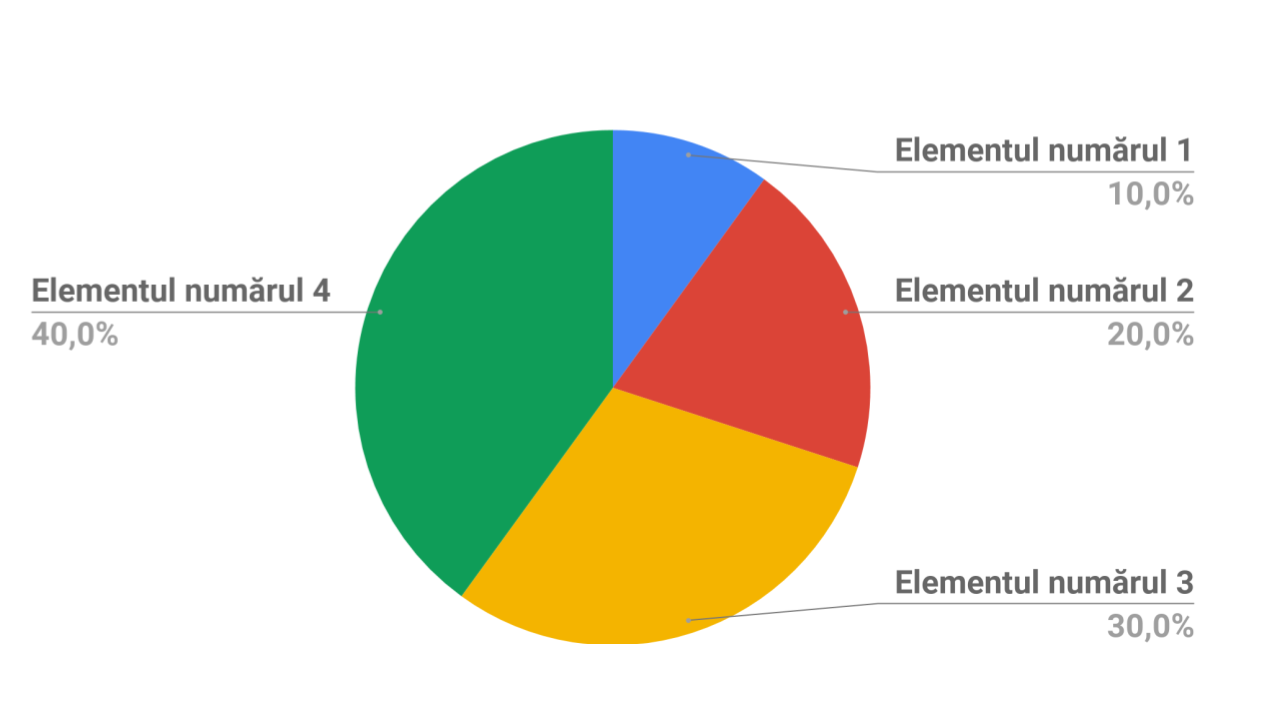
\includegraphics[	
		width=14cm,
		height=6cm,
		keepaspectratio
	]{imagini/probabilitati_selectie_ruleta.png}
	\caption{\textit{Probabilități de selecție ale elementelor.}}
	\label{fig:probabilitati_selectie_ruleta}
\end{figure}
		
Figura \ref{fig:probabilitati_selectie_ruleta} reprezintă un exemplu de ruletă divizată în patru sectoare de arii proporționale cu probabilitățile de selecție \cite{curs_daniela_zaharie}. Elementul numărul 1 are 10\% șanse de a fi selectat. Elementul numărul 2 are șanse de 20\%, numărul 3 de 30\% iar numărul 4 de 40\%.

\begin{figure}[H]
	\centering
	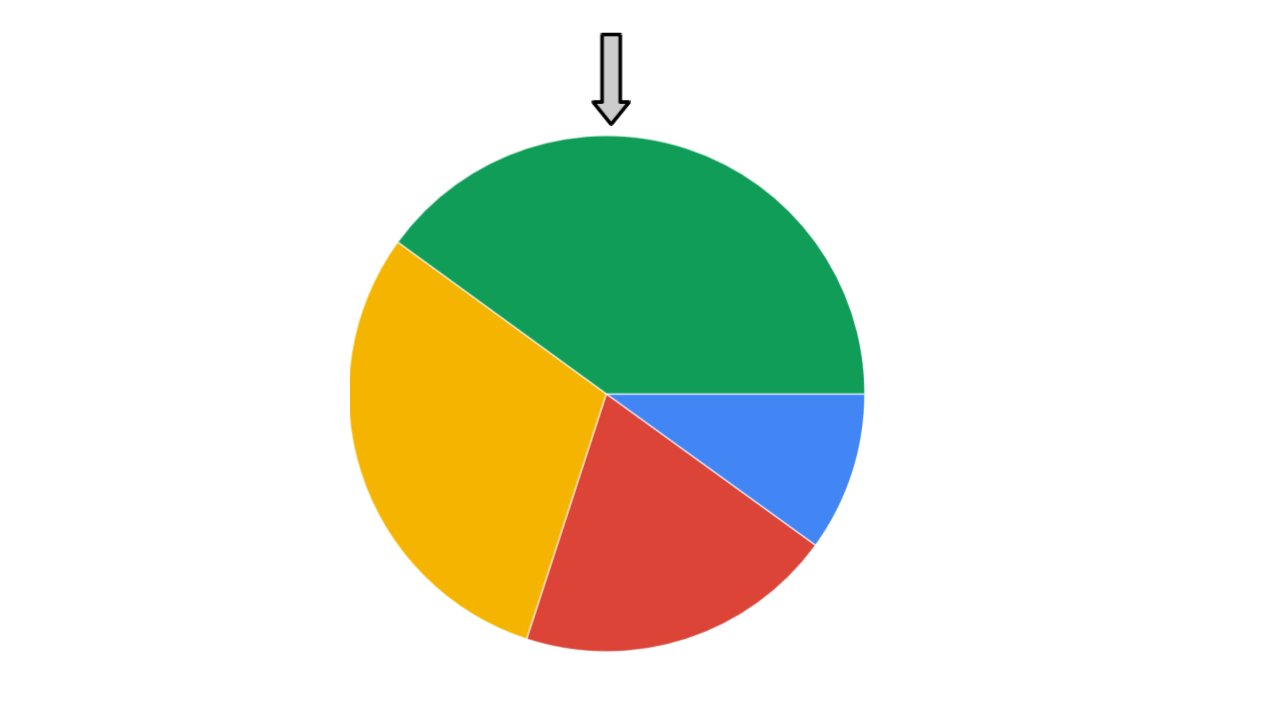
\includegraphics[	
		width=14cm,
		height=6cm,
		keepaspectratio
	]{imagini/invartire_ruleta.png}
	\caption{\textit{Rezultatul rotirii ruletei.}}
	\label{fig:invartire_ruleta}
\end{figure}

Rezultatul din Figura \ref{fig:invartire_ruleta} poate fi interpretat drept selectarea individului care corespunde categoriei etichetate cu verde (se alege elementul cu numărul 4, care a avut o probabilitate de selecție de 40\%).
